
\documentclass[11pt]{article}

% Geometry
\usepackage{fullpage}

% Ams math
\usepackage{amsmath}

% Include options such as \FloatBarrier
\usepackage{placeins}


% Include clickable links in the pdf
%\usepackage{hyperref}

% Packages for setting figures
\usepackage{graphicx}
\usepackage{caption}
\usepackage{subfig}
%\usepackage{subcaption}

\captionsetup[subfloat]{%
labelfont=bf,
font=small,}


% Tables
\usepackage{multirow}

\usepackage{enumerate}
\usepackage{color}

% Bibliography
\usepackage{natbib}

% Labels
\numberwithin{equation}{section}
\numberwithin{figure}{section}
\numberwithin{table}{section}
% http://tex.stackexchange.com/questions/42726/align-but-show-one-equation-number-at-the-end
\newcommand\numberthis{\addtocounter{equation}{1}\tag{\theequation}}


% Default image directory
\graphicspath{ {../InertialSpaceResults/img/}}

% tickz
\usepackage{amsmath}
\usepackage{tikz}

% Alter some LaTeX defaults for better treatment of figures:
    % See p.105 of "TeX Unbound" for suggested values.
    % See pp. 199-200 of Lamport's "LaTeX" book for details.
    %   General parameters, for ALL pages:
    \renewcommand{\topfraction}{0.9}	% max fraction of floats at top
    \renewcommand{\bottomfraction}{0.8}	% max fraction of floats at bottom
    %   Parameters for TEXT pages (not float pages):
    \setcounter{topnumber}{2}
    \setcounter{bottomnumber}{2}
    \setcounter{totalnumber}{4}     % 2 may work better
    \setcounter{dbltopnumber}{2}    % for 2-column pages
    \renewcommand{\dbltopfraction}{0.9}	% fit big float above 2-col. text
    \renewcommand{\textfraction}{0.07}	% allow minimal text w. figs
    %   Parameters for FLOAT pages (not text pages):
    \renewcommand{\floatpagefraction}{0.7}	% require fuller float pages
	% N.B.: floatpagefraction MUST be less than topfraction !!
    \renewcommand{\dblfloatpagefraction}{0.7}	% require fuller float pages



\begin{document}

\newcommand{\spin}{\boldsymbol{\omega}}
\newcommand{\m}{\hat{\boldsymbol{m}}}
\newcommand{\J}{\boldsymbol{J}}
\newcommand{\n}{\hat{\boldsymbol{n}}}
\newcommand{\V}{\boldsymbol{v}}

\title{Neutron star mechanics in the observers inertial frame}
\author{}
\maketitle
\section{Introduction}

In the rotating body frame we can solve Euler's rigid body equations to
calculate the motion of the spin vector $\spin$ as a function of time; this
allows observation of precession without resolving individual rotations on the
faster spin period. Observations of the star are made in the inertial frame and
so observers report on quantities calculable from the phase: timing residuals,
frequency of the the pulse and the spindown rate. In an effort to understand
the implications of precession on these quantities we aim to calculate the
motion of the star in the inertial frame.  A natural way to do this  is to
determine the Euler angles which transform the rotating body frame axis,
denoted by $(x',y', z')$, to the inertial frame axis for which we will use $(x,
y, z)$. Using the Euler angle parameterisation as described by
\citet{Landau1969} a schematic of how these angles are constructed is given in
figure \ref{fig:Euler}. 

\begin{figure}[ht]
\centering
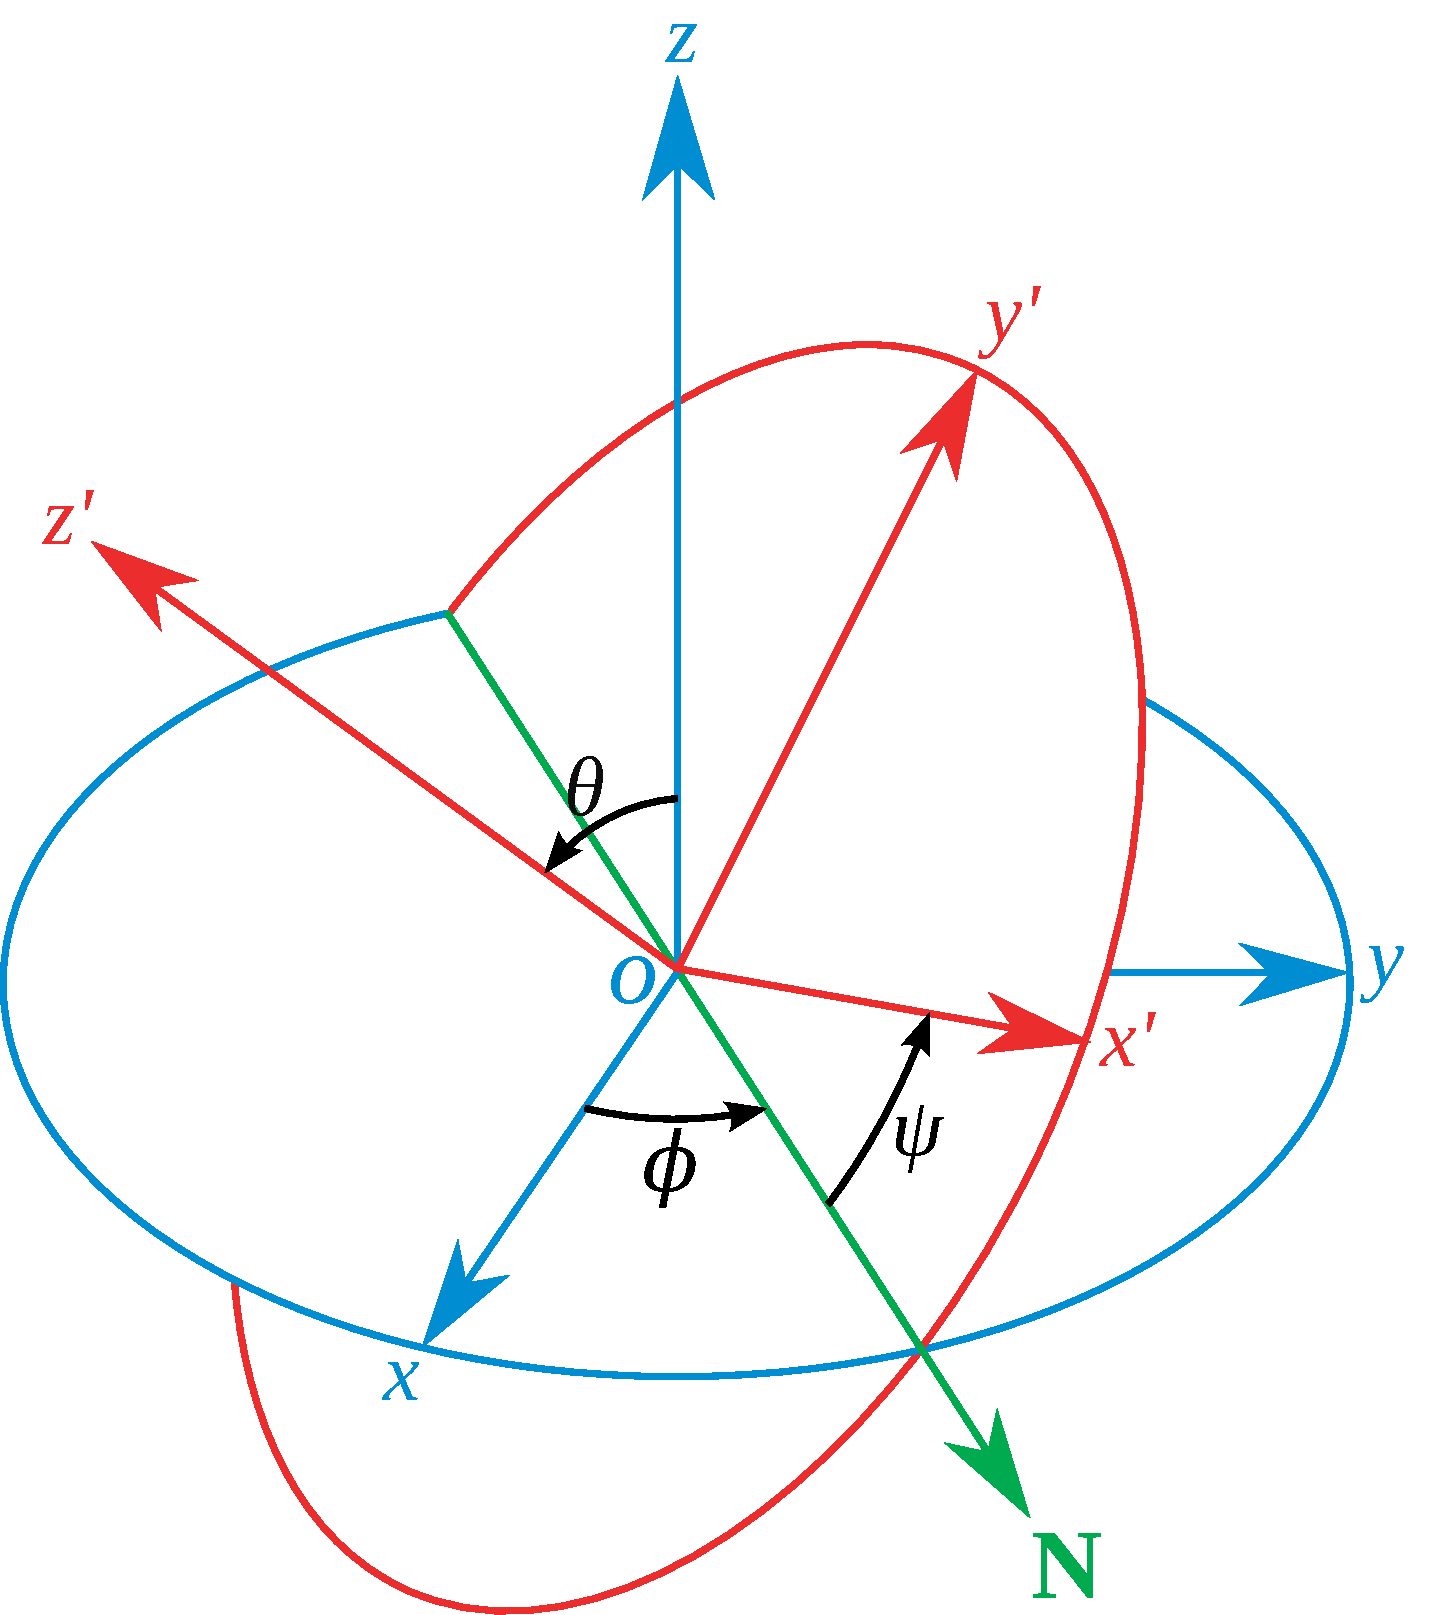
\includegraphics[scale=0.25]{Eulerangles-alternative.pdf}
% http://commons.wikimedia.org/wiki/File:Eulerangles-alternative.svg
\caption{Schematic of the Euler angle rotation. In the inertial frame the
angular momentum is set to lie initially along the $z$ axis. In the rotating
body frame for a biaxial body the deformation lies along $z'$ while the spin
vector initially lies along in the $x'- z'$ plane.}
\label{fig:Euler}
\end{figure}•

In the body frame we define the diagonal moment of inertia to have components
$I_{xx}$, $I_{yy}$ and $I_{zz}$ and acted upon by a torque $\boldsymbol{T}$. The
Euler rigid body equations are then the left most equations in
\eqref{eqn:ODEs}.
Decomposing the motion of the spin vector into Euler angles and rearranging
yields the second set of equations in \eqref{eqn:ODEs} for the rate of change
of the three Euler angles.

\begin{align*}
\dot{\omega_{x}} & = \frac{1}{I_{xx}}\left[T_{x}  + \left(I_{yy} - I_{zz}\right) \omega_{y} \omega_{z}\right],   &  
       \dot{\theta} & = \omega_{x} \cos \psi - \omega_{y} \sin \psi,
 \\
\dot{\omega_{y}} & =  \frac{1}{I_{yy}}\left[T_{y}  + \left(I_{zz} - I_{xx}\right) \omega_{x} \omega_{z}\right], & 
     \dot{\phi}  & = \frac{\omega_{x} \sin \psi + \omega_{y} \cos \psi}{\sin \theta}, 
\numberthis \label{eqn:ODEs}
\\
\dot{\omega_{z}} & =\frac{1}{I_{zz}}\left[T_{z}  + \left(I_{xx} - I_{yy}\right) \omega_{x} \omega_{y}\right],  & 
     \dot{\psi} & =  \omega_{z} - \dot{\phi} \cos \theta ,
\end{align*}

These equations can be solved numerically using a time stepper\footnote{For now
we will use the rkf45 stepper provided by GSL}. % Need reference
The rotation period of the star is several orders of magnitude smaller than the
precession period, as a result the Euler angles evolve on a much shorter time
scale than the body frame spin components. This is numerically expensive. To
allow efficient investigations we will therefore consider unrealistic values to
understand the different types of motion before using realistic values only in
cases of interest.

%Initially only torque free biaxial bodies are considered for simplicity, this
%system was studied by \citet{Jones2001} where it was demonstrated that for a
%biaxial body with deformation $\n_{d}$ along the $z'$ axis, this deformation,
%the spin vector and the angular momentum $\J$ are coplanar. They form a system
%which undergoes two different rotations: firstly at approximately the fast spin
%frequency the system rotates about $\J$ corresponding to a linear increase in
%$\phi$, then at the slower precession frequency the system counter rotates
%about $\n_{d}$ corresponding to a linear decrease in $\psi$ while $\theta$
%remains constant. This analytic example can be used to test the stability of
%numerical results before we go on to consider the effect of the torque and
%triaxiality. 

\section{Initial conditions}

Solving the rigid body equations in the body frame the following initial
conditions are imposed on the spin vector:

\begin{align}\label{eqn:spin init}
\omega_{x} & = \omega_{0}\sin(a_{0}), & 
\omega_{y} & = 0, & 
\omega_{z} & = \omega_{0}\cos(a_{0}),
\end{align}
such that  $\spin(t=0)$ lies in the $x' - z'$ plane. Defining the moment of
inertia and torque this is sufficient to solve the rigid body equations. The 
angular momentum vector in the two frames are related by the rotation matrix 
$R(\theta, \phi, \psi)$ constructed from the Euler angles
\begin{equation}
\left. \J \right|_{\textrm{Rot}} = R(\theta, \phi, \psi) \left. \J \right|_{\textrm{In} }
\label{eqn: transform}
\end{equation}•
The angular momentum in the inertial frame is given by $\left. \J
\right|_{\textrm{Rot}}= I \spin$, the initial conditions on $\spin$ then
provide initial conditions for the angular momentum.  BY setting an initial
condition on the angular momentum in the inertial frame we uniquely define the
inital Euler angles. We are free to set the initial angular momentum in the
inertial frame to lie along the inertial $z$ axis such that
$\left.\J_{0}\right|_{\textrm{I}} = |J|\hat{z}$. In the torque free case this
will remain true, the addition of the torque will induce variations.
Normalising the two vectors in equation \eqref{eqn: transform} and rearranging
gives the expression

\begin{equation}
\left[ \begin{array}{c}
\sin \psi_{0} \sin \theta_{0} \\
\sin \psi_{0} \cos \theta_{0} \\
\cos \theta_{0}
\end{array}\right]
 = \frac{1}{\sqrt{(I_{xx}\sin a_{0})^{2}  + (I_{zz}\cos a_{0})^{2}}} 
\left[ \begin{array}{c}
I_{xx}\sin a_{0} \\
0 \\
I_{zz} \cos a_{0}
\end{array}\right].
\end{equation}•

We have three equations for two unknowns; our choice to set $\J$ along
the $z$ axis leaves the initial value of $\phi$ a free variable, for simplicity
we set it to $\phi_{0} = 0$. Inserting this and comparing the components

\begin{equation}
\theta_{0} =  \arccos\left(\frac{I_{zz}\cos a_{0}}{ \sqrt{(I_{xx}\sin a_{0})^{2}  + (I_{zz}\cos a_{0})^{2}}} \right).
\label{eqn:theta init}
\end{equation} 

For $\psi_0$, we  use that $\sin(\arccos(x)) = \sqrt{1 - x^{2}}$ giving:

\begin{equation}
\psi_0 = \frac{\pi}{2}.
\end{equation}

We now have a suitable set of initial conditions to solve the 6 ODEs in \eqref{eqn:ODEs}.

\section{Biaxial body with no torque}

This system was studied by \citet{Jones2001} where it was  found that the
angular momentum $\J$, deformation axis $\n_{d}$\footnote{for a biaxial body we
    set $\n_{d}$ to lie along the $z'$ axis of the body frame} and spin vector
    $\spin$ are always coplanar. We will label this plane as the reference
    plane. Decomposing the angular velocity according to 

\begin{equation}
\spin = \dot{\phi}\n_{J} + \dot{\psi}\n_{d}
\label{eqn:decomp}
\end{equation}
it was found that $\phi$ monotonically increases at the  fast spin frequency whilst $\psi$ decreases at the slower precession frequency whilst $\theta$ should remain constant. 

Numerically solving the equations of motion these results are confirmed in figure \ref{fig:biaxial body no torque}(b) and also demonstrate the usual free precession in the body frame in \ref{fig:biaxial body no torque}(b):  the azimuthal angle $\varphi$ monotonically increases whilst the polar angle $a$ and the spin magnitude $\omega$ remain fixed. 

It is of note that in these simulations $\theta$ is not constant, this is caused by the finite numerical precision  when calculating the subtraction defined in equation \eqref{eqn:ODEs} for $\dot{\theta}=0$. On short time scales these errors have fractional size $1\times10^{-14}$ and so the results hold. Over sufficiently long time scale these errors can accumulate and  eventually leads to a complete loss of numerical accuracy, we must therefore be vigilant to ensure this does not occur when considering realistic values.
\begin{figure}[ht]
	\subfloat[Spherical components in the body frame]{\includegraphics[width=0.5\textwidth]{{Spherical_Plot_chi0_80.00_omega0_1.00e+01_epsI3_1.00e-03_n_10000_a0_15.00_T_5.00e+03_upsilon_0.000_epsA_0.00e+00_epsI1_0.00e+00_AnomTorque_1}.pdf}}
	\subfloat[Euler angles ]{\includegraphics[width=0.5\textwidth]
{{Euler_Angles_chi0_80.00_omega0_1.00e+01_epsI3_1.00e-03_n_10000_a0_15.00_T_5.00e+03_upsilon_0.000_epsA_0.00e+00_epsI1_0.00e+00_AnomTorque_1}.pdf}}
\caption{Solution to the differential equations in \eqref{eqn:ODEs} for a biaxial body with deformation of $\epsilon_{I3} = 1 \times 10^{-3}$}
\label{fig:biaxial body no torque}
\end{figure}•

\FloatBarrier
%\paragraph{Convergence test}
%To ensure that the small wobble in $\theta$, which should remain constant, is a numerical effect rather than a lack of physics we can plot the fractional size of the wobble whilst changing the absolute error tolerance given to the ODE stepping procedure. This is done in figure \ref{fig:error}
% \begin{figure}[ht]
%\centering
%\includegraphics[scale=0.4]{error_plot.pdf}
%\caption{Fractional size of variations in theta plotted against the relative error tolerance given to the stepper.}
%\label{fig:error}
%\end{figure}
%We observe a strange behaviour in which the magnitude of the fractional difference, defined by
%\begin{equation}
%\textrm{Var}(\theta) = \frac{\theta_{\textrm{max}} - \theta_{\textrm{min}}}{|\theta|},
%\end{equation}
%increases exponentially as the error becomes very small. This is due to a change in the type of variation of theta, for larger absolute errors we observe a period wobble around the expected value of $\theta$. In contrast for much smaller absolute errors the solution seems to wander of the mean value whilst also undergoing a periodic wobble. We demonstrate this in figure \ref{fig:error example} for the two extremes values. 
%
%\begin{figure}[ht]
%\centering
%\includegraphics[scale=0.4]{error_example.pdf}
%\caption{Resulsts of simulations with different error tolerances, interestingly the smaller absolute error produces greater numerical inaccuracy.}
%\label{fig:error example}
%\end{figure}

\FloatBarrier

\subsection{Physical observables}
Having the Euler angles allows us to transform from the rotating frame into the inertial frame of an exterior observer. We observe pulsars from the electromagnetic radiation that streams out along open field lines, while the mechanism is poorly understood in this model we will assume a thin columnated beam is emitted along the magnetic dipole $\m$. %Talk here about limitations this imposes 
In the body frame we set $\m$ at an angle $\chi$ to the $z'$ axis with unit vector $[\sin(\chi), 0, \cos(\chi)]$. Using the Euler angles to rotate this unit vector, the components in the inertial frame are given by:
\begin{equation}
\m = 
\left[\begin{array}{c}
\cos\phi\cos\psi\sin\chi - \sin\phi \cos \theta \sin \psi \sin \chi + \sin \phi \sin \theta \cos \chi \\
\sin\phi\cos\psi\sin\chi + \cos\phi \cos \theta \sin \psi \sin \chi - \cos \phi \sin \theta \cos \chi \\
\sin\theta \cos\psi \sin\chi + \cos\theta \cos \chi
\end{array}\right].
\label{eqn:m inertial}
\end{equation}•
Following the work of \citet{Jones2001} two angles $\Phi$ and $\Theta$ are defined to describe the polar and azimuth of $\m$ in the inertial frame. 
Defining $\Phi = \arctan(\m_{y} / \m_{x})$ after some algebra we arrive at: 
\begin{equation}
\Phi = \phi - \frac{\pi}{2} + \arctan\left(\frac{1}{\cos\theta}\left(\frac{\cos\psi \tan \chi}{\tan\theta - \sin \psi \tan\chi }\right)\right),
\label{eqn:Phi}
\end{equation}
while the polar angle of the magnetic dipole is given by:
\begin{equation}
\Theta = \arccos(\m_{z}) = \arccos(\sin \theta \sin \psi \sin \chi + \cos \theta \cos \chi )
\label{eqn:Theta}
\end{equation}
%An observers position can then also be described by the two spherical angles, for simplicity we will set the observer at $\Phi=0$ 
\paragraph{Instantaneous electromagnetic frequency}
An observer sees a pulse every time the magnetic dipole passes over them, making a simplification that a pulse is observed everytime the magnetic dipole cuts the plane containing the observer and the angular momentum vector $\J$. In effect we say the observer sees a pulse when the azimuth $\Phi$ is equal to their own regardless of the polar angle $\Theta$. In this way $\Phi$ gives the phase of the signal for an observer at $\Phi=0$ and $\Theta$ defines the amplitude being maximum when equal to that of the observer (who we place at $\Theta= 0$) . % Needs a better explanation
Taking a derivative of the phase:
\begin{equation}
\dot{\Phi} = \dot{\phi} 
+ \frac{\sin\chi \left(
\dot{\psi}  (\cos\theta\sin\chi - \sin \psi \sin \theta \cos\chi) + 
\dot{\theta} \cos\psi (\cos\theta\sin\chi - \sin \psi \sin \theta \cos\chi)\right) 
}{(\sin\theta \cos \chi - \cos \theta \sin \psi \sin \chi)^{2} + \cos^{2}\psi \sin^{2} \chi}.
\label{eqn:Phi_dot}
\end{equation}•
This is then the \emph{instantaneous electromagnetic frequency},  an observer will measure the time averaged value of $\dot{\Phi}$ as the 'spin frequency' of the star
Note that this result is an extension of equation (43) from \cite{Jones2001} treating $\theta$ as a function of time instead of a constant. Jones et al. demonstrated that two distinct behaviours exist  for the time average of equation \eqref{eqn:Phi_dot}. The two cases are catergoried by $\theta > \chi$ or $\theta < \chi$; recall that for the biaxial star with no torque $\theta \approx a_{0}$.

\subsection{Understanding the two cases}
To get a feeling for the mechanics we consider the decomposition of the angular velocity in equation \ref{eqn:decomp} into rotations about $\n_{J}$ and $\n_{d}$. Any vector (such as $\m$) in the body frame can be understood in the inertial frame as undergoing two motions: keeping $\phi$ fixed and increasing $\psi$ rotates the vector in a cone aboout the $\n_{d}$ axis, holding instead $\psi$ fixed and increasing $\phi$ sweeps the vector about a cone centered around the $\n_{J}$ axis.  Calling these cones the precession and spin cones respectively the resulting motion can be understood as the superposition of the two.  In figure \ref{fig:cones} an illustration is given of these cones projected into the reference plane for the three orderings of $\theta$ and $\chi$.  
\begin{figure}[ht]
\centering
	\subfloat[$\theta > \chi$]{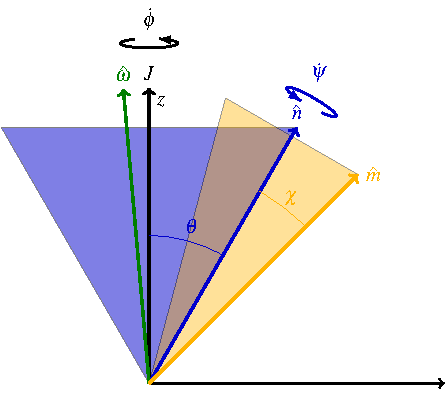
\includegraphics[width=0.33\textwidth]{chi_less_theta.pdf}}
	\subfloat[$\theta = \chi$]{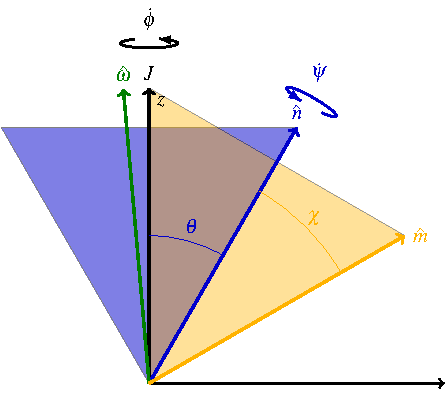
\includegraphics[width=0.33\textwidth]{chi_equal_theta.pdf}}
	\subfloat[$\theta < \chi$]{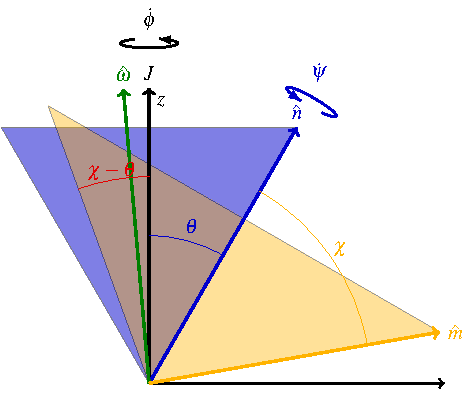
\includegraphics[width=0.33\textwidth]{chi_more_theta.pdf}}
\caption{Diagrams depiciting 2D projections of the cones swept out by the different motions under torque free precession onto the reference plane. The yellow cone is that swept out by $\m$ about $\n_{d}$ at the slow precession frequency; the blue cone is that swept out by $\n_{d}$ about $\J$ at the fast spin frequency. It should be noted that the precession cone rotates in the opposing direction to the spin cone for oblate bodies. }
\label{fig:cones}
\end{figure}

The motion of the magnetic dipole about the precession cone evolves on a much longer timescale than its motion about the spin cone, as a result the star will always pulsate once every spin period, but the long precession will induce variations.  Because of the large difference in timescales the motion of $\m$ can be considered as the slow evolution of a third cone swept out by $\m$ about $\J$ which we will call the dipole cone. The half angle made by this cone is exactly the azimuthal angle $\Theta$ calculated in equation \eqref{eqn:Theta}; the frequency with which $\m$ rotates in the dipole cone is given by equation \eqref{eqn:Phi_dot}, both these quantities will vary on the precession time scale. In figures \ref{fig:variations}(a) and (b) the frequency and polar angle variations are plotted for three particular cases, with reference to these plots we now discuss the three cases:
\begin{itemize}
\item The $\chi = \theta/2$ case: The precession cone is narrow and does not extend over the angular momentum vector. The polar angle $\Theta$ of the dipole cone then oscillates sinusoidally between $\theta+\chi$ and $\theta-\chi$ during a precession cycle. The spin frequency $\dot{\Phi}$ has an average value of $\dot{\phi}$\footnote{See Jones 2001 for a detailed explanation} and oscillates about this value, comparing with the $\Theta$ variations demonstrates these oscillations are locked in phase with the rotation of $\m$ in the precession cone. Recalling that the precession cone counter rotates with respect to the spin cone, at $\theta+\chi$ the precession cone motion acts in the opposing direction to the spin cone, this causes a reduction in the spin frequency away from the average; by contrast at $\theta+\chi$ the counter rotation is now in favour of the spin frequency and as a result the spin frequency is increased above the average.

\item The $\chi = \theta$ case: Here the angular momentum vector sits exactly on the precession cone, this suggest $\m$ can align exactly with the angular momentum. When this happens the spin frequency tends to zero (due to numerical error this never actually occurs) manifesting as sharp dips in the spin frequency; at the same time the polar angle tends to zero.

\item The $\chi = 4\theta$ case: The precession cone now extends over the angular momentum vector, this means it always acts to reduce the spin frequency; as a result the the spin frequency has an average value of $\dot{\phi} + \dot{\psi}$. The polar angle can vary between $\theta+\chi$ and $\chi-\theta$, for $\chi$ close to $\theta$ the deviations away from the average are large while as $\chi$ increases the deviations get smaller as thehalf angle of the dipole cone increases.
\end{itemize}•

\begin{figure}[ht]
\centering
	\subfloat[Variations in the spin frequency]{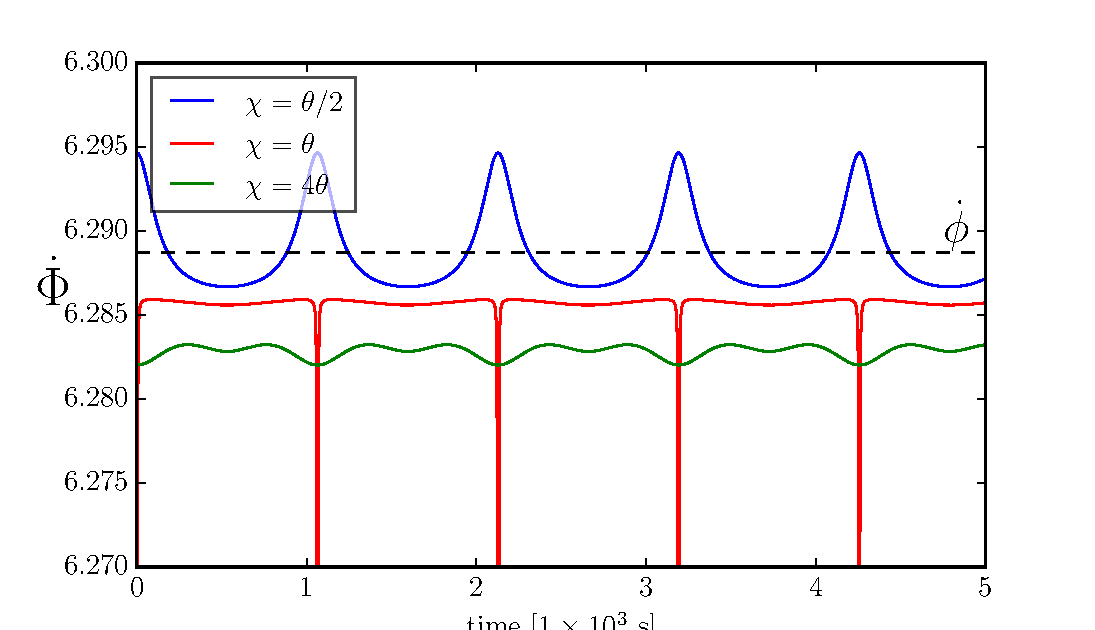
\includegraphics[width=0.7\textwidth]{frequency_variation_with_chi.pdf}} \\
	\subfloat[Variations in polar angle]{\includegraphics[width=0.7\textwidth]{amplitude_variation_with_chi.pdf}}
\caption{}
\label{fig:variations}
\end{figure}

\FloatBarrier
%\paragraph{Timing residuals}
%We now consider the timing residuals which would result from free precession alone. Clearly these are far from reality since the observed electromagnetic signal must act some torque on the body. Nevertheless, we can use equation \eqref{eqn:Phi} to calculate the exact phase of the signal. To compare with the tools used by observational astronomers we calculate the timing residual by fitting a third order Taylor series expansion to this phase. The residual is then the difference after subtraction
%
%\begin{figure}[ht]
%	\subfloat[$\chi<\theta$]{\includegraphics[width=0.5\textwidth]{{../../Timing_residuals/TR_chi_10.00}.png}}
%	\subfloat[$\chi > \theta$]{\includegraphics[width=0.5\textwidth]{{../../Timing_residuals/TR_chi_20.00}.png}}
%\caption{}
%\label{fig:}
%\end{figure}•

%\subsection{Biaxial body with torque}
%We now introduce the torque using the parameters of pulsar B1828-11 (Need to reference values here) to simulate a realistic pulsar making some assumptions on the cause of the periodic modulations. With realistic values the spin period is approximately a second, in comparison the precession period of the order of a year. The result is that we must resolve $10^{7}$ rotations of the neutron star per precessional orbit. 
%
%\begin{figure}[ht]
%	\subfloat[]{\includegraphics[width=0.5\textwidth]{{Spherical_Plot_chi_70.0_epsI1_0.00e+00_epsI3_9.37e-09_epsA_6.94e-12_omega0_15.51_aint_15_t1_3.00e+08}.pdf}}
%	\subfloat[]{\includegraphics[width=0.5\textwidth]{{Euler_Angles_chi_70.0_epsI1_0.00e+00_epsI3_9.37e-09_epsA_6.94e-12_omega0_15.51_aint_15_t1_3.00e+08}.pdf}}
%\caption{}
%\label{fig:}
%\end{figure}
\subsubsection{Timing residuals}
The principle indicator that a spin down power law does not accurately describe the evolution of pulsars is the coherent structure which exists in the timing residuals. We now aim to introduce the tools required to calculate the timing residuals from our model and determine what effect, if any, torque free precession will induce. 

Starting with the instantaneous electromagnetic frequency as given by equation \eqref{eqn:Phi_dot} % should we explain why we cant just use phi?
and numerically integrating yields the phase of the pulse, we will label this $\Phi_{\textrm{exact}}$, a quadratic polynomial is then fitted to this phase using a least squares method. The resulting coefficients, $\dot{\nu}, \nu$ and $\phi_{0}$ are the physical quantities best describing the results for a power law spin down. Calculating the phase according to this polynomial gives $\Phi_{\textrm{fit}}$ the fitted phase. The difference between these two phases is the timing residual as calculated by observers. 

In figure \ref{fig:TR no torque} we plot the timing residuals as calculated in the torque free model while changing the inclination of the magnetic dipole. It is worth noting that there is an issue in doing this, namely the power law spin down assumes that the star is in fact spinning down; without the torque this model will not spin down. We can however interpret these results as the effect of precession on timing residuals in the limit for which the variation due to precession is much stronger than the spin down.% ($\tau_{p} \ll \tau_{s}$

\begin{figure}[ht]
\centering
	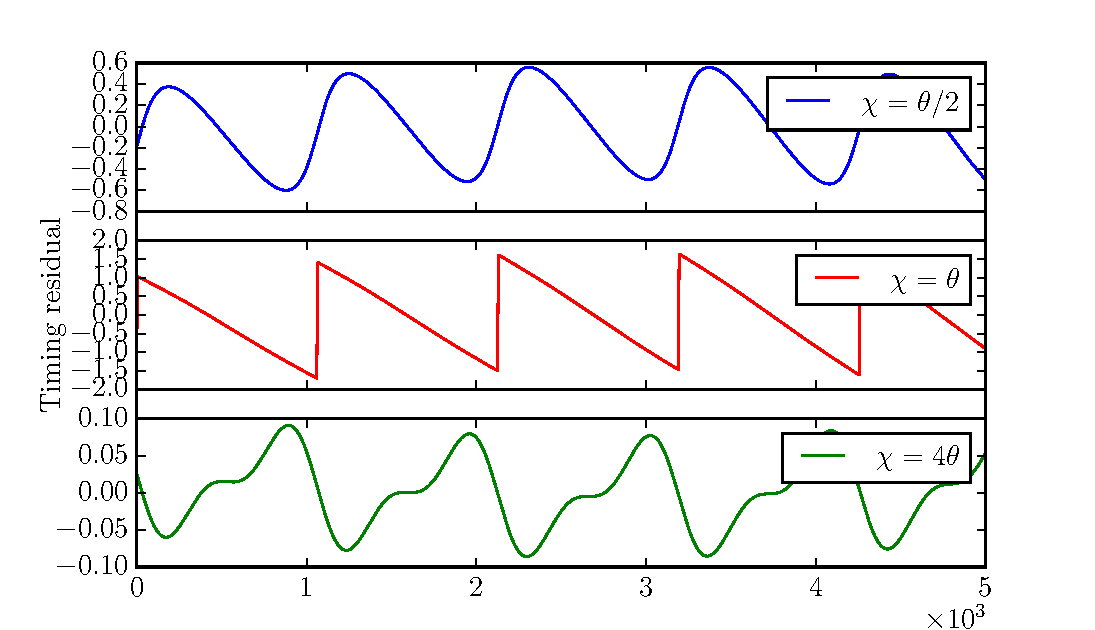
\includegraphics[width=0.7\textwidth]{Timing_residuals_no_torque.pdf}
\caption{Plot of the timing residuals for various angles of $\chi$ in the torque free model. }
\label{fig:TR no torque}
\end{figure}

The results show that the precession will induce a sinusoidal variation on the precession timescale, the magnitude is proportional to the angle $\chi$, there will also be a dependence on the initial angle $a_{0}$ as this is a geometric effect.

\subsection{Slowdown Rate $\dot{\nu}$}
The second observable which is often considered in characterising periodic patterns in pulsar signals is the slowdown rate. In this simple model the slowdown rate is given by $\ddot{\Phi}$, however calculating an analytic expression is highly non-trivial, although theoretically possible. Instead of relying on computational aids to achieve this we instead turn to the method prescribed by \citet{Lyne2010}: selecting short sections of data of length $T$ a quadratic is fitted allowing an estimation of $\dot{\nu}$, this process is repeated every $\sim T/4$ through the data set. We choose $T$ such that it is a fraction of the precession period over which we expect quantities to be modulated. To aid the eye the values have been normalised and plotted in figure \ref{fig:nu_dot no torque}. This has the advantage that any features resulting from the technique will also be picked up.
\begin{figure}[ht]
\centering
	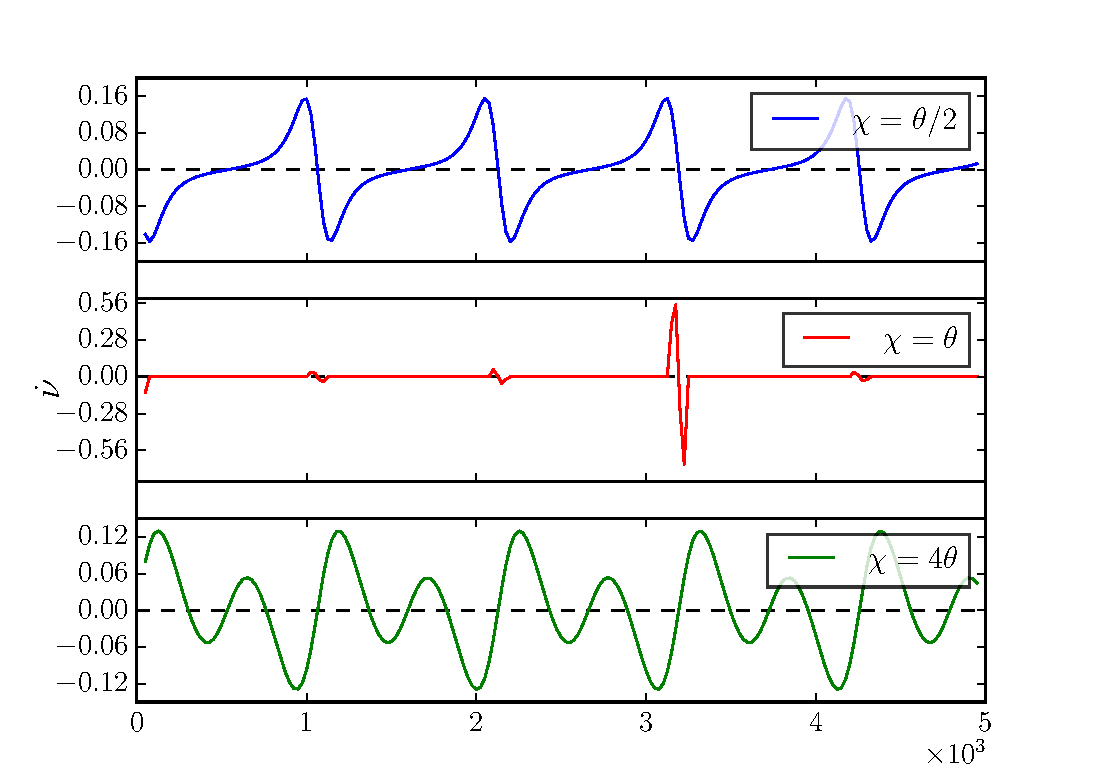
\includegraphics[width=0.7\textwidth]{nu_dot_no_torque.pdf}
\caption{Slow down rate }
\label{fig:nu_dot no torque}
\end{figure}

\section{Biaxial body with torque}
The torque which produce the observed electromagnetic radiation will play an important role in determining the time variability of the observed pulse on earth. The torque is modelled as a magnetic dipole, denoted by $\m$, frozen into the star at an angle $\chi$ to the $z'$ axis in the $x'-z'$ plane. Following the work of \citet{Deutsch1955}, the torque is presented here in form found in \citet{Goldreich1970}.
\begin{equation}
\boldsymbol{T}=\frac{2R}{3c} I_{0}\epsilon_{A}\omega^{2}(\boldsymbol{\omega} \times \hat{\boldsymbol{m}})\times \hat{\boldsymbol{m}} + \epsilon_{A}I_{0}(\boldsymbol{\omega} \cdot \hat{\boldsymbol{m}})(\boldsymbol{\omega} \times \hat{\boldsymbol{m}}), \;\;\;\;\; \textrm{ with } \;\;\;\; \epsilon_{A} = \frac{m^{2}}{I_{0}R_{6}c^{2}},
\label{eqn:torque}
\end{equation}
where $\boldsymbol{\omega}$ is the spin vector and $\epsilon_{A}$ is the magnetic deformation \citep[see][]{Glampedakis2010}.
The first term on the right hand side is often referred to as the \emph{spin down}, or \emph{braking} torque. As this suggests it is responsible for the power law retardation of spin frequency and has an associated timescale $\tau_{S}$. The second term is known as the \emph{anomalous} torque which acts on a timescale $\tau_{A}$. Inserting this torque into the ODEs defined in \eqref{eqn:ODEs} then we have three time scales: the two due to the torque stated above and the precession time scale $\tau_{P}$ as found by \citet{Jones2001}. These three timescales are given by:
\begin{align}
\tau_{P} &= \frac{1}{\epsilon_{I}\nu_{0}},  &  \tau_{A}&=\frac{1}{\epsilon_{A}\nu_{0}}, & \tau_{S}&=\frac{3c}{2R}\frac{1}{\epsilon_{A}\nu_{0}^{2}},
\label{eqn:timescales}
\end{align} 
where $\nu_{0}$ is the initial spin frequency and $\epsilon_{I}$ is the magnitude of the elastic deformation along $z$ ($I_{zz} = I_{xx} + \epsilon_{I}$). In previous work we have shown % Maybe include this?
that realistic pulsars exist in the region $\tau_{P} > \tau_{A}$ for which $\epsilon_{A} < \epsilon_{I}$, in order to demonstrate the effect of the torque we will work for $\epsilon_{A} = \epsilon_{I}/2$. 
\subsection{Results}
In figure \ref{fig:biaxial body with torque} we plot the spherical components of the spin vector in the body frame (a), and the evolution of the Euler angles. Comparing this with figure \ref{fig:biaxial body no torque} the most striking difference is the wobble in both $\theta$ and $a$, on closer inspection one also finds this wobble in the other angles and the magnitude of $\spin$ along with a monotonic spin down.

\begin{figure}[ht]
	\subfloat[]{\includegraphics[width=0.5\textwidth]{{Spherical_Plot_chi0_80.00_omega0_1.00e+01_epsI3_1.00e-03_n_10000_a0_15.00_T_5.00e+03_upsilon_0.000_epsA_5.00e-04_epsI1_0.00e+00_AnomTorque_1}.pdf}}
	\subfloat[]{\includegraphics[width=0.5\textwidth]{{Euler_Angles_chi0_80.00_omega0_1.00e+01_epsI3_1.00e-03_n_10000_a0_15.00_T_5.00e+03_upsilon_0.000_epsA_5.00e-04_epsI1_0.00e+00_AnomTorque_1}.pdf}}
\caption{Solution to the differential equations in \eqref{eqn:ODEs} including the torque defined in  \eqref{eqn:torque} for a biaxial body with $\epsilon_{A}=\epsilon_{I}/2$ }
\label{fig:biaxial body with torque}
\end{figure}•

\FloatBarrier
\subsection{Observables}
In figure \ref{fig:variations with torque} we reproduce plots of figure \ref{fig:variations} with the addition of the torque. The torque introduces two additional effects: $\dot{\Phi}$ the instantaneous electromagnetic frequency  decays slowly, this is caused by the spin down torque and is full agreement with what we expect; a fast sinusoidal oscillation in $\dot{\Phi}$ on the spin time scale, observable as a broadening of the line, is a result of the anomalous torque. As for the polar angle $\Theta$ the anomalous torque causes slight changes in the limits of the sinusoidal variation. Both the anomalous torque effects can be understood by realising that this effectively adds a triaxiality into the moment of inertia tensor. % needs more explanation

\begin{figure}[ht]
\centering
	\subfloat[Variations in the spin frequency]{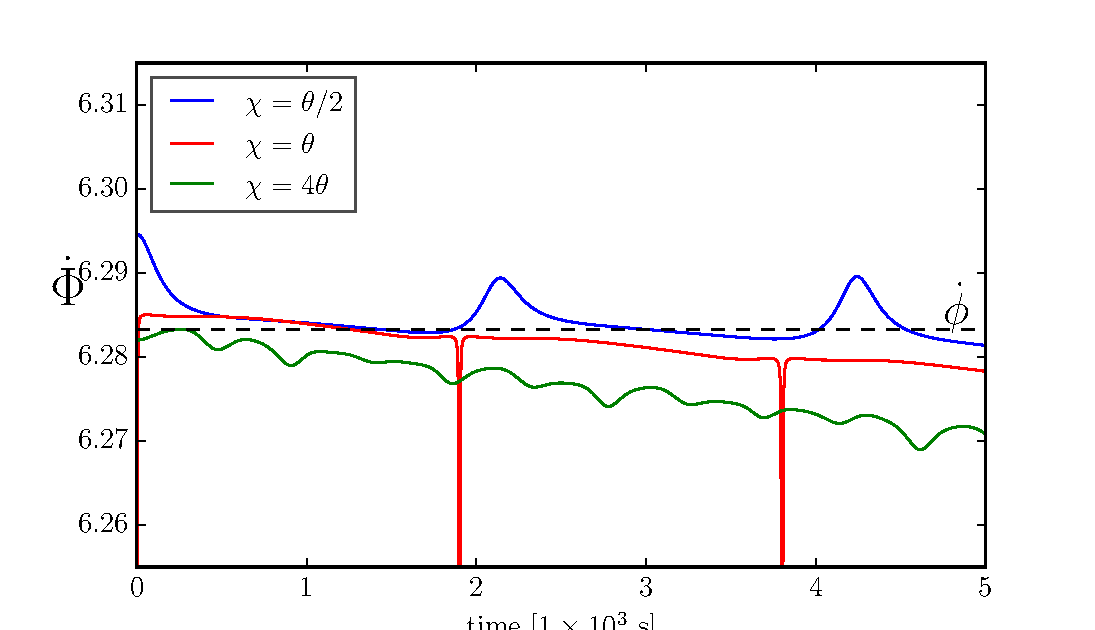
\includegraphics[width=0.7\textwidth]{frequency_variation_with_chi_inc_torque.pdf}} \\
	\subfloat[Variations in polar angle]{\includegraphics[width=0.7\textwidth]{amplitude_variation_with_chi_inc_torque.pdf}}
\caption{}
\label{fig:variations with torque}
\end{figure}

\FloatBarrier
\subsubsection{Timing residual}
Including the torque the timing residuals are plotted in figure \ref{fig:TR with torque}, while the sinusoidal variation remains the magnetic inclination varies the spin down rate and hence the period of the these variations.
\begin{figure}[ht]
\centering
	\subfloat[No anomalous torque ]{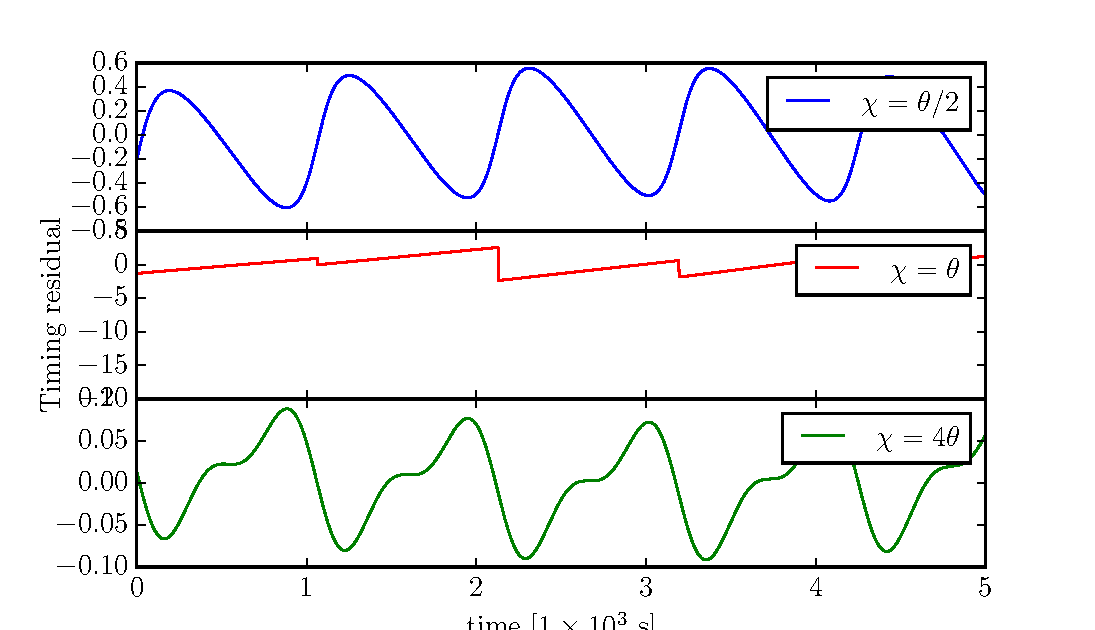
\includegraphics[width=0.6\textwidth]{Timing_residuals_with_torque_no_anom.pdf}} \\
	\subfloat[With anomalous torque]{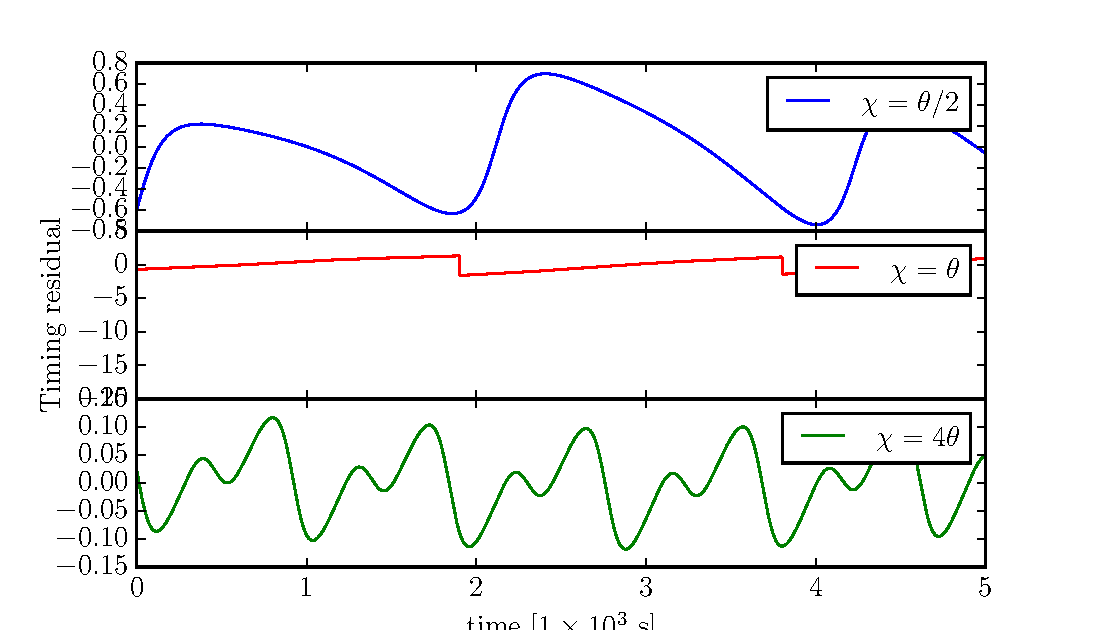
\includegraphics[width=0.6\textwidth]{Timing_residuals_with_torque.pdf}}

\caption{Plot of the timing residuals for various angles of $\chi$ including the effects of the torque. }
\label{fig:TR with torque}
\end{figure}

\FloatBarrier
\subsection{Slowdown Rate $\dot{\nu}$}


\begin{figure}[ht]
\centering
	\subfloat[No anomalous torque ]{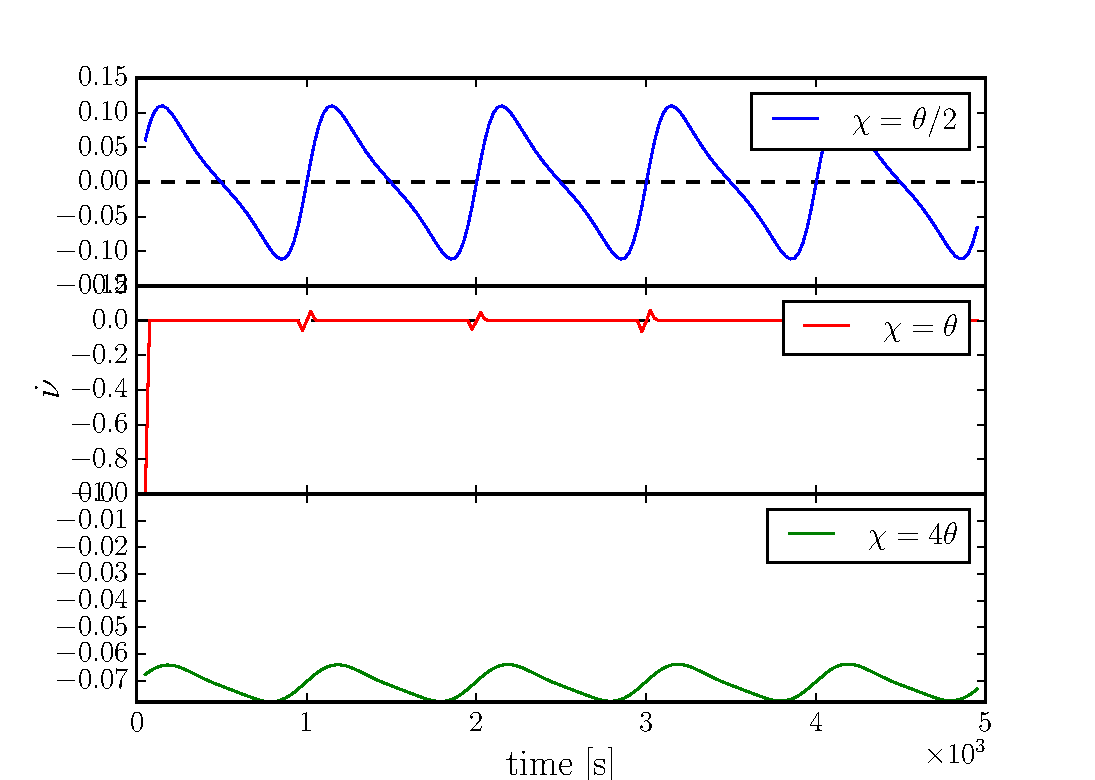
\includegraphics[width=0.6\textwidth]{nu_dot_with_torque_no_anom.pdf}} \\
	\subfloat[With anomalous torque]{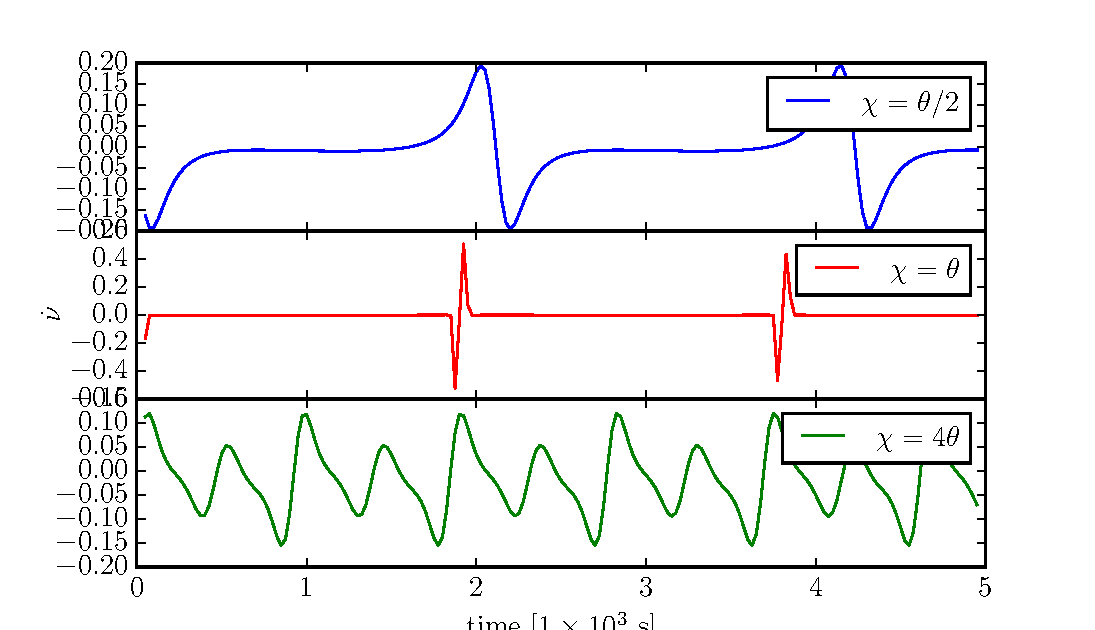
\includegraphics[width=0.6\textwidth]{nu_dot_with_torque.pdf}}
\caption{}
\label{fig:nu_dot no torque}
\end{figure}



\FloatBarrier
\section{B1828-11}
In order to compare the prediction of our model with actual observations we select the pulsar B1828-11. There is some evidence in work by \cite{Lyne2000} that this pulsar undergoes precession,  and work by \cite{Hobbs2010} and \cite{Lyne2010} documents the timing residuals and spin down rate with unsurpassed accuracy. This makes the pulsar ideal for study under the assumption that the variations are caused by precession.

From table 1 in \citet{Lyne2000} we have that B1828-11 has  a spin period of $P_{0}=405$ms. We can calculate the magnetic deformation using the surface magnetic field 
\begin{equation}
\epsilon_{A}=\frac{m^{2}}{I_{0}Rc^{2}}=\frac{(\frac{1}{2}B_{s}R^{3})^{2}}{I_{0}Rc^{2}}
\end{equation}
From table1 we have that $B_{s}=5\times10^{12}$G and using canonical values of $R$, $c$ and $I_{0}$\footnote{Should I give the actual values?} yields $\epsilon_{A}=6.94\times10^{-12}$.

For the elastic deformations we have an upper limit from gravitational wave searches of $1\times10^{-6}$. We now make the assumption that it is precession which causes the variations in signal, from \citet{Jones2001} we may therefore use that 
\begin{equation}
\epsilon_{I} \sim  \frac{P_{\textrm{spin}}}{P_{\textrm{precession}}}
\end{equation}•
Lyne found timescales of 1000, 500 and 250 days for the variations, we will use the shortest of these such that $P_{precession}=250$ days. Hence we have an elastic deformations of $1.88 \times10^{-8}$. This also agrees well with \citet{Lyne2010} B1812-11 is observed for $\sim6000$ days during which 22 oscillations occur, this gives a period of about $273$ days. 
With these values we have the following timescales
\begin{equation*}
\tau_{S}=1.06\times10^{15} \textrm{ s} \;\;\;\; \;\;\;\; \tau_{A}=5.83\times10^{10} \textrm{ s} \;\;\;\; \;\;\;\; \tau_{P}=3.55\times10^{6} \textrm{ s}
\end{equation*}•

No obvious way exists to define $\chi$ other than to assume it must not be aligned on grounds that we can observe the pulsar. Since this pulsar satisfies the region A conditions and is therefore subject to the critical of $\chi$ we again choose the two values of $\chi$ previously used.
\FloatBarrier
%\section{Torque switching effects}
%\citet{Lyne2010} found strong evidence that a periodic switching in the rate of spin down $\dot\nu$ induces structure in the residual. Modeling this they found that for a strictly periodic switching the variations are precisely mirrored in the residual, if instead a random dither is introduced between switches the residuals take form very similar to those found in \citet{Hobbs2010}. The model assumes apriori that the switching occurs with a time scale of several 100 days, the switching itself is motivated by changes in the magnetosphere: enhances emmison correlates with larger values of $\dot\nu$. A mechanism is required to keep the magnetosphere in serveral meta-stable states with swithing occuring on a much shorter time scale than the period between swithces. \citet{Jones2010} % is that right?
%proposed that if the star were to be precessing, its relative orientation to the angular momentum may bias it towards different magneospheric configurations. Stars born near the boundary between configurations will then periodially flip between them on the precession timescale which matches well with the observed switching times. In this section we aim to model this proposal by extending our model; this is done by adding a switching into the torque that depends on the angle $\Psi $ between $\m$ and the angular momentum. As previously shown this angle is bounded by $|\chi - \theta| < \Psi < \chi + \theta$ during a precessional cycle, it therefore has an average value of $\Psi_{\textrm{ave}}\max(\theta, \chi)$; while many different scenarios could be considered we choose the following: 
%\begin{equation}
%\boldsymbol{S}(\Psi, \chi, \theta, \upsilon) = \left\{
%\begin{array}{ccc}
%1 & \textrm{if} & \Psi > \Psi_{\textrm{ave}} \\
%1 - \upsilon & \textrm{else} & 
%\end{array}•\right. 
%\end{equation}
%where $\upsilon$ is a number between 0 and 1 parameterising the reduction in torque. 
%
%To illustrate the effect this can have we use a value of $\upsilon=0.8$ 
%
%\begin{figure}[ht]
%\centering
%	\subfloat[ ]{\includegraphics[width=0.55\textwidth]{../../Testing/switching_euler_angles.pdf}} 
%	\subfloat[]{\includegraphics[width=0.55\textwidth]{../../Testing/switching_big_theta.pdf}} \\
%	\subfloat[ ]{\includegraphics[width=0.55\textwidth]{../../Testing/switching_timing_residual.pdf}} 
%	\subfloat[]{\includegraphics[width=0.55\textwidth]{../../Testing/switching_nu_dot.pdf}} \\
%\caption{}
%\label{fig:switching}
%\end{figure}
%
%\FloatBarrier
%\appendix
%\section{Euler angles}
%\begin{equation}
%\left[\begin{smallmatrix}- \sin{\left (\phi \right )} \sin{\left (\psi \right )} \cos{\left (\theta \right )} + \cos{\left (\phi \right )} \cos{\left (\psi \right )} & \sin{\left (\phi \right )} \cos{\left (\psi \right )} + \sin{\left (\psi \right )} \cos{\left (\phi \right )} \cos{\left (\theta \right )} & \sin{\left (\psi \right )} \sin{\left (\theta \right )}\\- \sin{\left (\phi \right )} \cos{\left (\psi \right )} \cos{\left (\theta \right )} - \sin{\left (\psi \right )} \cos{\left (\phi \right )} & - \sin{\left (\phi \right )} \sin{\left (\psi \right )} + \cos{\left (\phi \right )} \cos{\left (\psi \right )} \cos{\left (\theta \right )} & \sin{\left (\theta \right )} \cos{\left (\psi \right )}\\\sin{\left (\phi \right )} \sin{\left (\theta \right )} & - \sin{\left (\theta \right )} \cos{\left (\phi \right )} & \cos{\left (\theta \right )}\end{smallmatrix}\right]
%\label{eqn:rotation matrix}
%\end{equation}•
%
%
%\section{Catastrophic cancellation}
%The ODEs defined in \eqref{eqn:ODEs} suffer a 

\bibliographystyle{apalike}	
\bibliography{../bibliography}
\end{document}

